\documentclass[pdf, blends]{prosper}
\usepackage[utf8]{inputenc}
%\usepackage[latin1]{inputenc}
\usepackage[spanish]{babel}
\usepackage{color}
\usepackage{amsmath}
\usepackage{graphicx}
\usepackage{graphics}
\usepackage{multicol} 
\usepackage{listings}
\lstset{ %
language=C++,                % choose the language of the code
basicstyle=\footnotesize,       % the size of the fonts that are used for the code
numbers=left,                   % where to put the line-numbers
numberstyle=\footnotesize,      % the size of the fonts that are used for the line-numbers
stepnumber=1,                   % the step between two line-numbers. If it is 1 each line will be numbered
numbersep=5pt,                  % how far the line-numbers are from the code
backgroundcolor=\color{black},  % choose the background color. You must add \usepackage{color}
showspaces=false,               % show spaces adding particular underscores
showstringspaces=false,         % underline spaces within strings
showtabs=false,                 % show tabs within strings adding particular underscores
frame=single,   		% adds a frame around the code
tabsize=2,  		% sets default tabsize to 2 spaces
captionpos=b,   		% sets the caption-position to bottom
breaklines=true,    	% sets automatic line breaking
breakatwhitespace=false,    % sets if automatic breaks should only happen at whitespace
escapeinside={\%}{)}          % if you want to add a comment within your code
}
\title{Ecuaciones Diferenciales Parciales Parabólicas}
\subtitle{Curso de Física Computacional}
\author{M. en C. Gustavo Contreras Mayén}
\email{curso.fisica.comp@gmail.com}
%\ptsize{11}
\begin{document}
\maketitle
\begin{slide}{Problema}
Hay una barra de longitud $L=100$ cm y de diámetro $w$ (vista desde el eje $x$). La barra está aislada en su perímetro, excepto los extremos.
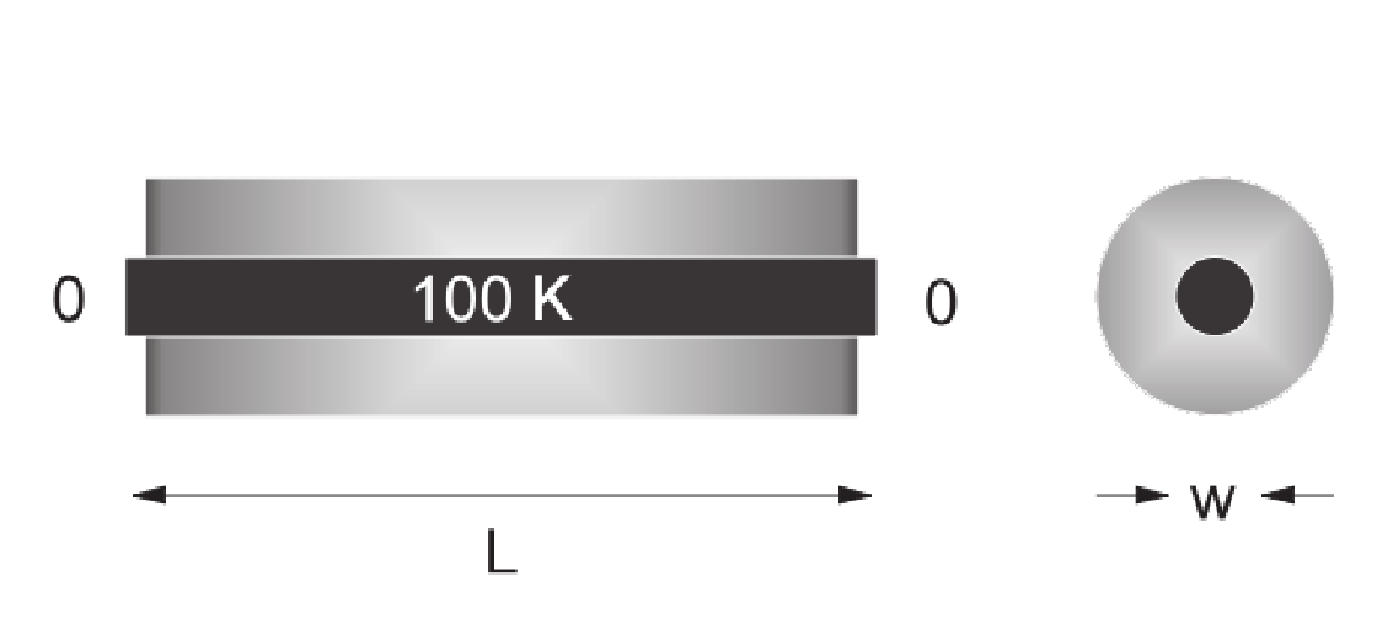
\includegraphics[scale=0.4]{EjemploEqCalor.eps} 
\end{slide}
\begin{slide}{\ptsize{10} 2}
Al inicio la barra cuenta con una temperatura uniforme de $100^{\circ}$ C y los extremos de la misma están en contacto con agua helada. El calor fluye hacia los extremos que no están dentro del aislante.
\\
El problema a resolver es: estimar cómo varía la temperatura a lo largo de la barra para un instante de tiempo dado, además de ver cómo cambia con respecto al tiempo.
\end{slide}
\begin{slide}{Ecuación de calor}
¿Cómo es el flujo de calor de una región caliente a una región fría?
\\
Expresando el fenómeno en términos matemáticos:  decimos que la razón de cambio de flujo de calor $\mathbf{H}$ a través de un material, es proporcional al gradiente de temperatura $T$ en el material.
\[ \mathbf{H} = -k \nabla T(\mathbf{x},t)  \]
donde $k$ es la conductividad térmica del material.
\end{slide}
\begin{slide}{Breviario 1}
La cantidad total de calor $Q(t)$ en cualquier momento, es proporcional a la  integral de la temperatura sobre del volumen del material:
\[ Q(t) = \int d\mathbf{x} C \rho (\mathbf{x}) T(\mathbf{x},t) \]
Donde $C$ es el calor específico del material y es $\rho$ la densidad del material. 
\end{slide}
\begin{slide}{Breviario 2}
Dado que la energía se conserva, la razón de decremento de $Q$ con el tiempo debe de ser igual a la cantidad de calor fluyendo fuera del material. 
\\
Después de que tenemos este balance de energía y aplicamos el teorema de la divergencia, la ecuación de calor, resulta:
\[ \dfrac{\partial T(\mathbf{x},t)}{\partial t} = \dfrac{k}{C \rho} \nabla^{2} T(\mathbf{x},t) \]
Suponemos que la densidad $\rho$ del material es constante.
\end{slide}
\begin{slide}{Breviario 3}
Tenemos una EDP de tipo parábolico con variables independientes de posición y tiempo. 
\\
Especificar este tipo de problema implica que no hay variación de la temperatura en las direcciones perpendiculares de la barra $(y,z)$, por lo que sólo tenemos una coordenada espacial:
\[ \dfrac{\partial T(\mathbf{x},t)}{\partial t} = \dfrac{k}{C \rho} \nabla^{2} T(\mathbf{x},t) \]
\end{slide}
\begin{slide}{De nuevo al problema}
La temperatura inicial de la barra y las condiciones de frontera son:
\begin{eqnarray*}
T(x,t=0) & = & 100^{\circ} \\
T(x=0, t) = T(x=L,t) & = & 0^{\circ} 
\end{eqnarray*}
\end{slide}
\begin{slide}{Solución numérica}
Como se revisó con la ecuación de Laplace, la solución numérica se basa en convertir una ecuación diferencial en una aproximación por diferencias finitas.
\\
\\
El algoritmo se desarrolla a partir de expandir $T(x,t+\Delta t)$ y $T(x+\Delta x,t)$ en series de Taylor, dejándo los términos de menor orden en $\Delta$:
\end{slide}
\begin{slide}{Desarrollo en series de Taylor}
\begin{equation*}
T(x, t + \Delta t) \simeq T(x,t) + \dfrac{\partial T (x,t)}{\partial t} \Delta t }
\end{equation*}
\begin{equation*}
T(x + \Delta x,t) \simeq T(x,t) +  \dfrac{\partial T}{\partial x} \Delta x}
\end{equation*}
\begin{equation*}
\Longrightarrow \dfrac{\partial T(x,t)}{\partial t} \simeq \dfrac{T(x, t + \Delta t)- T(x,t)}{\Delta t}
\end{equation*}
\begin{equation*}
\dfrac{\partial^{2} T(x,t)}{\partial x^{2}} \simeq \dfrac{T(x+\Delta x,t) + T(x-\Delta x,t)- 2 T(x,t)}{(\Delta x)^{2}}
\end{equation*}
\end{slide}
\begin{slide}{Continua la solución}
La EDP se transforma en una ecuación de diferencias finitas:

\end{slide}
\end{document}